% Obligatoire ! Spécifie le type de document avec parmi les options possibles le
% format papier et la taille de police par défaut
\documentclass[a4paper,11pt]{scrbook}

%        1         2         3         4         5         6          7         8
%%%%%%%%%%%%%%%%%%%%%%%%%%%%%%%%%%%%%%%%%%%%%%%%%%%%%%%%%%%%%%%%%%%%%%%%%%%%%%%%%
%                                                                               %
%                                 PREAMBULE                                     %
%                                                                               %
%%%%%%%%%%%%%%%%%%%%%%%%%%%%%%%%%%%%%%%%%%%%%%%%%%%%%%%%%%%%%%%%%%%%%%%%%%%%%%%%%

%%%%%%%%%% Pour gérer la langue (par défaut : anglais) %%%%%%%%%%
\usepackage[francais]{babel}
\usepackage[utf8]{inputenc}
\usepackage[T1]{fontenc}

%%%%%%%%%% Pour enrichir les possibilités de mise en forme ... %%%%%%%%%%
% ... des équations
\usepackage{amssymb,amsmath,amsthm}
% ... des algorithmes
\usepackage[ruled,vlined]{algorithm2e}

%%%%%%%%%% Pour enrichir les éléments de mise en page %%%%%%%%%%
\usepackage{minitoc, footmisc}

%%%%%%%%%% Pour enrichir les possibilités de mise en page du texte %%%%%%%%%%
\usepackage{helvet, courier, type1cm}
% Pour faire apparaitre joliment du code dans le rapport
\usepackage{listings}
% Pour enrichir les possibilités de mise en forme des légendes
\usepackage[small]{caption}

%%%%%%%%%% Pour enrichir les possibilités de mise en page des figures %%%%%%%%%%
\usepackage{graphicx}
% Pour spécifiee les chemins par défaut où aller chercher les figures
\graphicspath{{./figures/intro/}}
\usepackage{color}
\definecolor{blackgreen}{rgb}{0,0.4,0}

%%%%%%%%%% Pour enrichir les possibilités de mise en forme des annexes %%%%%%%%%%
\usepackage{appendix}

%%%%%%%%%% Modification de la mise en page par défaut %%%%%%%%%%
%\addtolength{\hoffset}{1cm}
\addtolength{\voffset}{-.5cm}
\addtolength{\textheight}{1cm}
%\addtolength{\textwidth}{0.5cm}

%%%%%%%%%% Modification des ENTETEs ET PIEDs DE PAGE par défaut %%%%%%%%%%
\usepackage{fancyhdr}
\pagestyle{fancy} \fancyhf{}
\fancyhead[RE]{\nouppercase{\textit{\leftmark}}} 	% Right even
\fancyhead[LO]{\nouppercase{\textit{\rightmark}}} 	% Left odd
\fancyhead[LE]{\textbf{\thepage}}			% Left even
\fancyhead[RO]{\textbf{\thepage}}	 		% Left even
\renewcommand{\footrulewidth}{0pt}
\setlength{\headheight}{50pt}
\setlength{\oddsidemargin}{30pt}  	% Marge gauche sur pages impaires
\setlength{\evensidemargin}{0pt} 	% Marge gauche sur pages paires


%%%%%%%%%% Mise en forme des liens %%%%%%%%%%
\usepackage[colorlinks=true, linkcolor=blue, citecolor=blue, urlcolor=blue]{hyperref} %, breaklinks=true


%%%%%%%%%%%%%%%%%%%%%%%%%%%%%%%%%%%%%%%%%%%%%%%%%%%%%%%%%%%%%%%%%%%%%%%%%%%%%%%%%
%                                                                               %
%               Configuration de certaines commandes                            %
%                                                                               %
%%%%%%%%%%%%%%%%%%%%%%%%%%%%%%%%%%%%%%%%%%%%%%%%%%%%%%%%%%%%%%%%%%%%%%%%%%%%%%%%%

% Gestion de la mise en forme du code (Cf. la doc du package listings)
\lstset{language=C, %C
%
basicstyle=\ttfamily\scriptsize,        % la taille de la police de caractère utilisée pour le code
keywordstyle=\color{red}\textbf,	% le style des mots clés du langage
commentstyle=\color{blue},		% le style des commentaires
%
numbers=left,                   	% où mettre les numéros de ligne
numberstyle=\ttfamily\scriptsize, 	% le style des numéros de ligne
numberblanklines=false,
%
captionpos=t,                   % place la légende en bas
frame=TB,	                %
%
showspaces=false,               % affichage des espaces
showstringspaces=false,         % affichage des chaines de caractères
showtabs=false,                 % affichage des tabulations dans les chaines de caractères
tabsize=4,	                % taille d'une tabulation
%
moredelim=[s][\color{blackgreen}]{'}{'},
moredelim=[s][\color{blackgreen}]{"}{"},
}

%%%%%%%%%%%%%%%%%%%%%%% Définition de commandes et de raccourcis personnalisés %%%%%%%%%%%%%%%%%%%%%%
\newcommand{\tens}[1]{#1}
\providecommand{\vect}[1]{\mbox{\boldmath${#1}$}}%$
\newcommand{\argmin}[1]{\underset{#1}{\operatorename{argmin}}}
\newcommand{\diag}{\mathop{\mathrm{diag}}}
\newcommand{\norm}[1]{\ensuremath{\left\lVert #1 \right\rVert}}

\renewcommand{\frame}[1]{\ensuremath{\Psi_{#1}}}	%frame				\Psi_{\uppercase{#1}}
\newcommand{\R}[1]{\ensuremath{\mathbb{R}^{#1}}}	%R for real
\newcommand{\Id}[1]{\ensuremath{\tens{I}_{#1}}}		%Identity matrix
\newcommand{\tp}{\ensuremath{^{\mathsf{T}}}}		%transpose
\newcommand{\ft}[2]{\ensuremath{_{#1,#2}}} 			%from to
\newcommand{\rt}[1]{\ensuremath{^{#1}}}				%relative to		%transpose
\newcommand{\HM}{\ensuremath{\tens{H}}}				%homogenous matrix
\newcommand{\Rot}{\ensuremath{\tens{R}}}			%rotation matrix
\newcommand{\homo}[1]{\ensuremath{\widetilde{#1}}}	%homogeneous coordinate
\renewcommand{\skew}[1]{\ensuremath{\widehat{#1}}}	%skew-matrix related to a vector
\newcommand{\pt}[1][p]{\ensuremath{\vect{#1}}}		%point in space
\newcommand{\ve}[1][u]{\ensuremath{\vect{#1}}}		%vector in space
\newcommand{\force}{\ensuremath{\vect{f}}}			%force
\newcommand{\torque}{\ensuremath{\vect{\tau}}}		%torque
\newcommand{\ttorque}{\ensuremath{\tau}}			%torque for subscript

\newcommand{\Eq}[1]{Eq.(\ref{#1})}
\newcommand{\Eqs}[2]{Eqs.(\ref{#1})--(\ref{#2})}
\newcommand{\Equation}[1]{Équation~(\ref{#1})}
\newcommand{\Problem}[1]{Problème~(\ref{#1})}
\newcommand{\Algo}[1]{Algorithme~(\ref{#1})}
\newcommand{\Algos}[2]{Algorithmes~(\ref{#1})--(\ref{#2})}
\newcommand{\Fig}[1]{Fig.~\ref{#1}}
\newcommand{\Figs}[2]{Figs.~\ref{#1}~\&~\ref{#2}}
\newcommand{\Figure}[1]{Figure~\ref{#1}}
\newcommand{\Sec}[1]{Section~\ref{#1}}
\newcommand{\Chapter}[1]{Chapitre~\ref{#1}}
\newcommand{\Chapters}[2]{Chapitres~\ref{#1}--\ref{#2}}
\newcommand{\Appendix}[1]{Annexe~\ref{#1}}
\newcommand{\Sections}[2]{Sections~\ref{#1}--\ref{#2}}
\newcommand{\Table}[1]{Table~(\ref{#1})}




%%%%%%%%%%%%%%%%%%%%%%%%%%%%%%%%%%%%%%%%%%%%%%%%%%%%%%%%%%%%%%%%%%%%%%%%%%%%%%%%%
%                                                                               %
%                             DEBUT DU DOCUMENT                                 %
%                                                                               %
%%%%%%%%%%%%%%%%%%%%%%%%%%%%%%%%%%%%%%%%%%%%%%%%%%%%%%%%%%%%%%%%%%%%%%%%%%%%%%%%%

\begin{document}
%-------------------------  Gestion des tables des matières et numérotations  -------------------------%
\frontmatter
\setcounter{tocdepth}{3}
\setcounter{secnumdepth}{3}

%------------------------------------> Page de titre
\begin{titlepage}
%----------------------------------------------------------------------------
% cover
%----------------------------------------------------------------------------
\thispagestyle{empty}
\addtolength{\hoffset}{-.5cm}
%\addtolength{\textwidth}{.5cm}
%\addtolength{\voffset}{-.5cm}
\addtolength{\textheight}{1cm}
\begin{center}
{\large \bf ENSEIRB-ENSC\\}
\vspace{5pt}
{\large \bf Parcours Robotique et Apprentissage\\}
\vfill
{\Huge Projet Robotique}
\vfill
\vspace{15pt}
travail réalisé par
\vfill
{\large \bf Kloé Bonnet et Guillaume Lauga}
\vfill
\rule[2mm]{60mm}{0.2mm}\\
{\huge Rapport de projet : Titre du projet\\}
\rule[-2mm]{60mm}{0.2mm}\\
\vfill
\textit{Année universitaire 2024 - 2025}
\vfill
\vspace{30pt}
{\bf Encadrement}
\vspace{10pt}
{\small
\begin{tabular}{p{0.05\textwidth}p{.40\textwidth}p{.55\textwidth}}
 & & \\
Titre &  Prénom {\sc Nom}  & Fonction\\
 & & \\
\end{tabular}
}
\end{center}

\end{titlepage}
\newpage
\thispagestyle{empty}
\null

%------------------------------------> Résumé
\chapter*{Résumé}
\thispagestyle{empty}

Lorem ipsum dolor sit amet, consectetur adipiscing elit. Duis et tellus ut dui tristique lacinia vel at leo. Praesent cursus accumsan mauris, vitae pulvinar dolor blandit id. Nullam sit amet sem vel elit porta tempus. Pellentesque scelerisque tellus et ligula volutpat porta. Nunc accumsan, augue porttitor eleifend tincidunt, mauris tortor interdum velit, vehicula gravida mauris felis sed dolor. Nullam eget elit metus, nec ultrices enim. Sed bibendum, nibh et eleifend malesuada, neque nisi blandit arcu, eget adipiscing nisi quam sed ligula. Pellentesque imperdiet dictum ultrices. Pellentesque habitant morbi tristique senectus et netus et malesuada fames ac turpis egestas.

Praesent in turpis ligula. Cras convallis condimentum quam in consectetur. Etiam iaculis nisi ac justo tempus pellentesque. Class aptent taciti sociosqu ad litora torquent per conubia nostra, per inceptos himenaeos. Nunc eleifend nunc vel lacus tempor sagittis ut in massa. Quisque semper varius tellus. Duis ornare auctor libero, in iaculis ante mollis ac.

Vivamus enim augue, malesuada eget bibendum sed, pharetra eleifend lacus. Curabitur elit justo, varius eget iaculis in, iaculis vel leo. Nulla vulputate felis urna. Donec faucibus, velit nec congue faucibus, ligula turpis consectetur arcu, ut faucibus nisi nunc vitae eros. Donec ut congue ipsum. Nullam blandit risus nec massa convallis malesuada. Nullam fringilla elementum neque, gravida adipiscing nulla scelerisque non.

Aenean elementum adipiscing elit vitae fermentum. Praesent vel pretium justo. Cras vel nibh ac lorem sollicitudin malesuada. Proin malesuada, erat in ullamcorper facilisis, mauris justo vehicula augue, id euismod quam nisi vitae magna. Vestibulum ut risus massa, vel euismod risus. Curabitur in blandit libero. Aliquam eleifend nisl sit amet lacus viverra ut malesuada enim venenatis. In sodales, sapien id feugiat adipiscing, quam nisl sagittis augue, ut scelerisque mi purus in justo. In ullamcorper rutrum magna, a tincidunt neque eleifend eu.

Phasellus tempus facilisis justo eu lobortis. Vestibulum vitae sem sed ante dictum commodo. Aenean nisi quam, sollicitudin a mattis vitae, auctor nec lorem. Integer convallis nunc ut leo imperdiet quis consequat magna semper. Nunc euismod laoreet neque in volutpat. Integer augue lectus, sodales a rutrum a, congue nec velit. Pellentesque nisi enim, placerat et ultricies sollicitudin, tempor ac risus. Nullam condimentum, tellus id elementum semper, nisl odio cursus odio, eu mollis sapien ipsum nec sapien. Vivamus eget porta lectus.


\vfill
\noindent
\textbf{Mots-clés: }\emph{Blabli, Blablo, Blublu.}

%------------------------------------> Table des matières
\tableofcontents

%------------------------------------> Liste des figures
\listoffigures
\addcontentsline{toc}{chapter}{\listfigurename}

%-------------------------  Corps du rapport  -------------------------%
\mainmatter

%#####################################################################################
%#####################################################################################
%#####################################################################################
\chapter*{Introduction}
% Ajoute un chapitre non numéroté à la table des matières
\addcontentsline{toc}{chapter}{Introduction}

Les règles de base de construction d'un rapport doivent être respectées. Par exemple, les éléments suivants ne sont pas facultatifs :
\begin{itemize}
\item respect des règles grammaticales, orthographiques et syntaxiques de la langue choisie pour écrire le rapport; cette langue est soit le français soit l'anglais;
\item la page de garde doit préciser au minimum le titre, l'année, le contexte (Option Robot,...), le nom des réalisateurs et les encadrants du projet;
\item présence d'une table des matières ou d'un sommaire;
\item présence d'une introduction et d'une conclusion.
\end{itemize}

L'introduction d'un rapport se compose généralement de plusieurs parties strictement nécessaires:
%une liste à puces
\begin{itemize}
\item la présentation du contexte du travail réalisé et faisant l'objet du rapport;
\item les enjeux du problème traité;
\item les travaux existants ayant déjà traité tout ou partie du problème en question;
\item les limites de ces travaux;
\item les contributions du travail présenté dans le rapport au regard des problèmes ouverts évoqués avant;
\item le plan du rapport.
\end{itemize}


Concernant le style du rapport, quelques règles élémentaires doivent elles aussi être respectées :
%une liste numérotées
\begin{enumerate}
\item un rapport technique s'écrit de manière impersonnelle et il faut donc éviter d'employer les termes \textit{je, nous, on};
\item un rapport présente des faits intemporels et le temps à préférer est le \textbf{présent de l'indicatif}. Le passé et le futur ne doivent généralement pas être utilisés;
\item toute figure telle la \Figure{fig:intro_figure} doit être citée dans le corps du texte; il en va de même pour les références bibliographiques tel que \cite{Oetiket} dans laquelle est proposé une courte introduction à \LaTeX;
\item deux titres ne peuvent se suivre sans être séparés par du texte. Par exemple, le titre d'un chapitre ne peut pas être directement suivi du titre d'une section. Les deux doivent être séparés par un texte introduisant le chapitre en question;
\item tout mot d'une langue qui n'est pas celle choisie pour le rapport doit apparaître en italique. En outre toute abbréviation ou tout sigle doit être systématiquement défini lors de sa première utilisation.
\item Il faut choisir une convention pour la représentation des scalaires, des vecteurs et des matrices. Une convention souvent utilisée est la suivante :
	\begin{itemize}
	\item scalaire : lettres minuscules;
	\item vecteurs : lettres minuscules grasses;
	\item matrices : lettres majuscules.
	\end{itemize}
\item Les équations sont des éléments du discours comme les autres et n'échappent donc pas aux règles de la ponctuation. Ainsi le polynôme $p$ défini comme
\begin{equation}
p(x) = \sum_{i=0}^n a_i x^i, \label{equ:poly}
\end{equation}
où $x \in \mathbb{R}$, $i \in \mathbb{N}$ et $a_i \in \mathbb{R}$, fait partie de la phrase. L'équation~(\ref{equ:poly}) est ponctuée en conséquence. Toutes les notations et nouveaux symboles, doivent par ailleurs être correctement introduits, en précisant, le cas échéant, les unités de certaines grandeurs.
\item Les graphiques et courbes doivent être, tels que celui présenté sur la figure~\ref{fig:resimpact}, correctement légendés, en précisant notamment les unités pour chacun des axes.
\item Le découpage en chapitre, section, sous-section, ... doit-être équilibré\footnote{contrairement à ce qui est proposé avec cet exemple}.
\end{enumerate}

% Insertion d'une figure
% Le placement des figures est automatique
\begin{figure*}
\centering
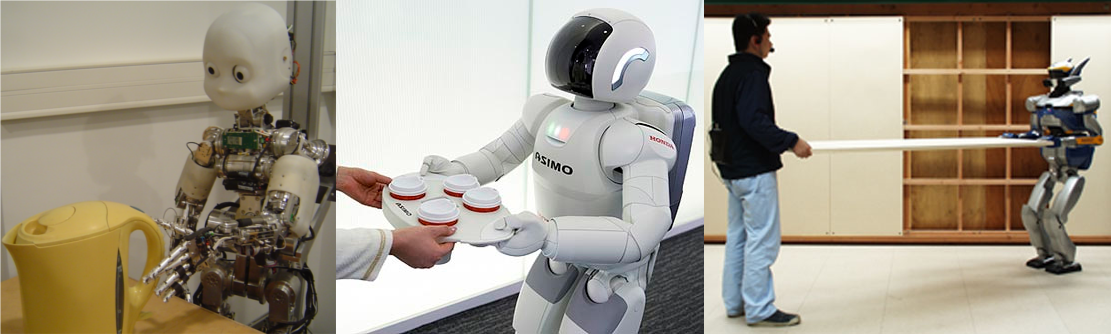
\includegraphics[width=\textwidth]{several_humanoids.png}
\caption[Un texte résumant la légende]{La légende en version plus longue. Elle s'affiche sous la figure et doit être suffisament descriptive (ce qui n'est pas le cas ici). Source: ISIR/Sorbonne Université, Honda Research,AIST/CNRS JRL \label{fig:intro_figure}}
\end{figure*}

\begin{figure*}
	 \centering
	 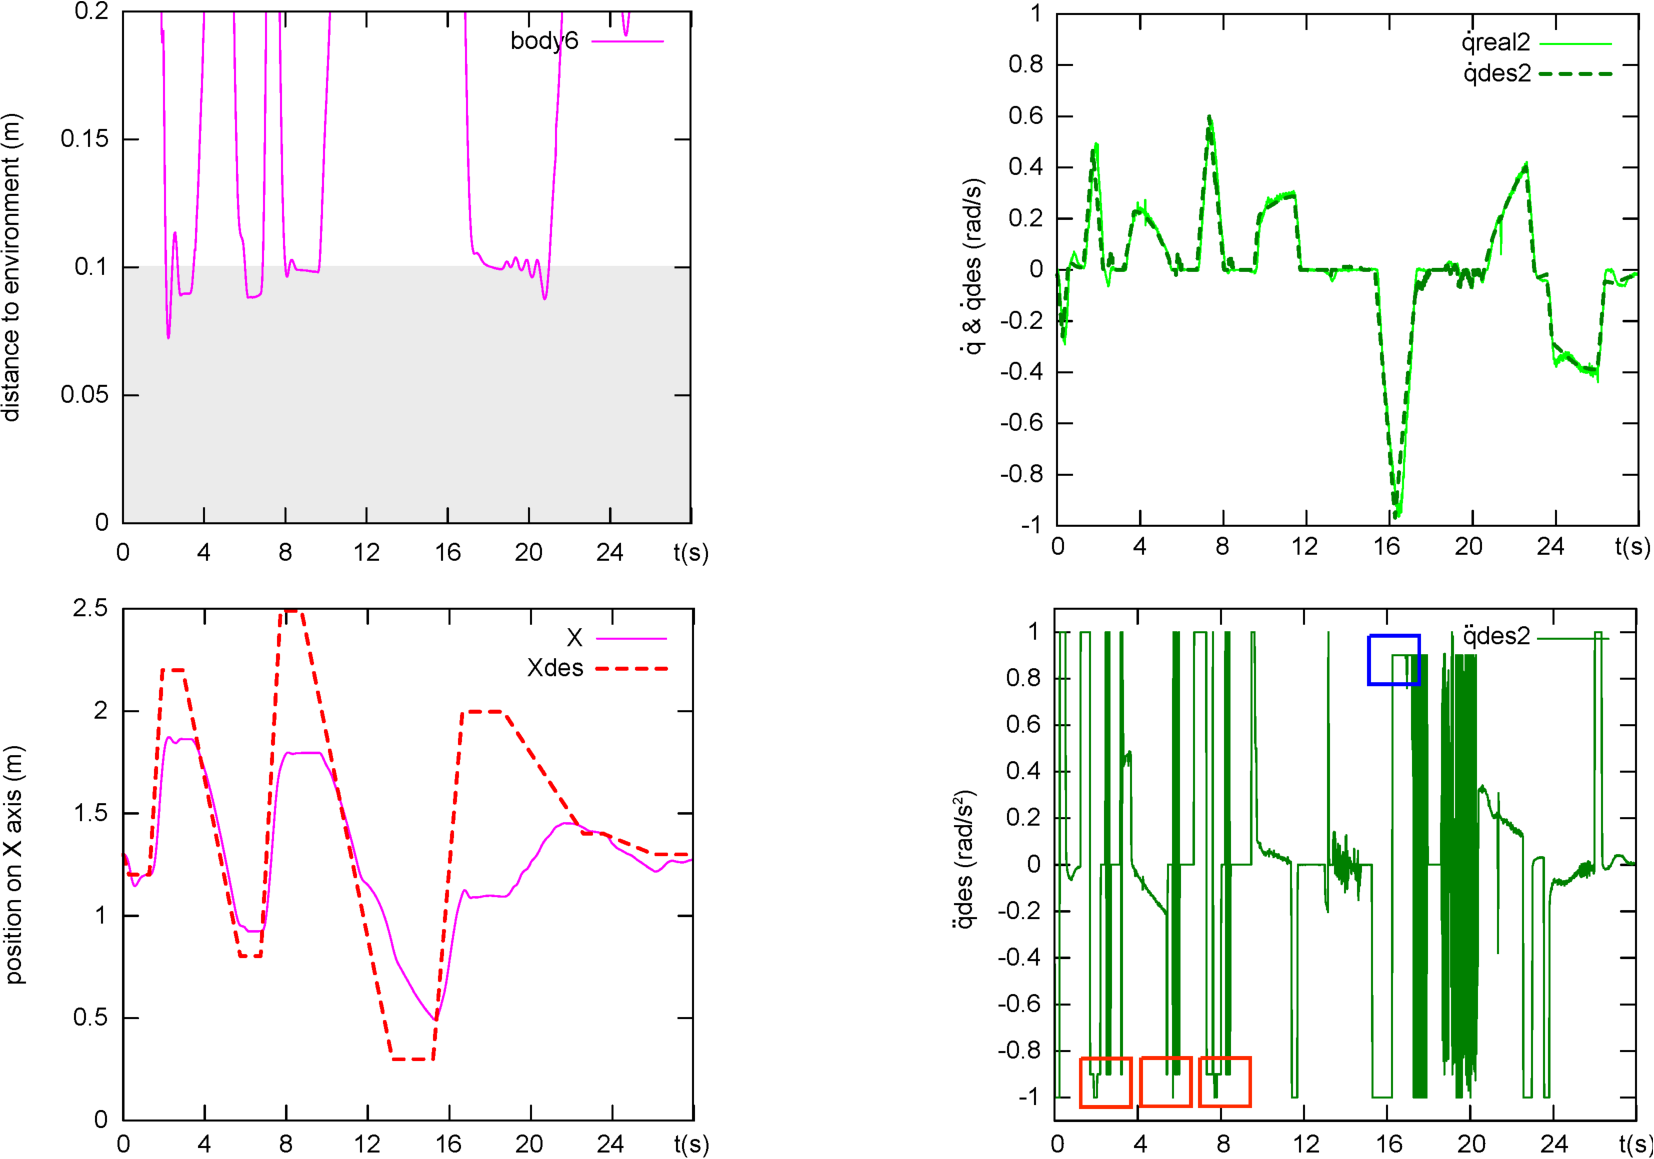
\includegraphics[width=0.85\textwidth]{figure11.pdf}
	 \caption{Results of experiment 2. \textit{Left column}: shortest distance between body 6 and the environment, desired and real position along Cartesian axis X; \textit{right column}: desired and real velocity of joint 2, accelerations of joint 2. Tiré de \cite{rubrecht-AutonomousRobots2012}.}
	 \label{fig:resimpact}
\end{figure*}

Lorem ipsum dolor sit amet, consectetur adipiscing elit. Duis et tellus ut dui tristique lacinia vel at leo. Praesent cursus accumsan mauris, vitae pulvinar dolor blandit id. Nullam sit amet sem vel elit porta tempus. Pellentesque scelerisque tellus et ligula volutpat porta. Nunc accumsan, augue porttitor eleifend tincidunt, mauris tortor interdum velit, vehicula gravida mauris felis sed dolor. Nullam eget elit metus, nec ultrices enim. Sed bibendum, nibh et eleifend malesuada, neque nisi blandit arcu, eget adipiscing nisi quam sed ligula. Pellentesque imperdiet dictum ultrices. Pellentesque habitant morbi tristique senectus et netus et malesuada fames ac turpis egestas.

Praesent in turpis ligula. Cras convallis condimentum quam in consectetur. Etiam iaculis nisi ac justo tempus pellentesque. Class aptent taciti sociosqu ad litora torquent per conubia nostra, per inceptos himenaeos. Nunc eleifend nunc vel lacus tempor sagittis ut in massa. Quisque semper varius tellus. Duis ornare auctor libero, in iaculis ante mollis ac.

Vivamus enim augue, malesuada eget bibendum sed, pharetra eleifend lacus. Curabitur elit justo, varius eget iaculis in, iaculis vel leo. Nulla vulputate felis urna. Donec faucibus, velit nec congue faucibus, ligula turpis consectetur arcu, ut faucibus nisi nunc vitae eros. Donec ut congue ipsum. Nullam blandit risus nec massa convallis malesuada. Nullam fringilla elementum neque, gravida adipiscing nulla scelerisque non.

Aenean elementum adipiscing elit vitae fermentum. Praesent vel pretium justo. Cras vel nibh ac lorem sollicitudin malesuada. Proin malesuada, erat in ullamcorper facilisis, mauris justo vehicula augue, id euismod quam nisi vitae magna. Vestibulum ut risus massa, vel euismod risus. Curabitur in blandit libero. Aliquam eleifend nisl sit amet lacus viverra ut malesuada enim venenatis. In sodales, sapien id feugiat adipiscing, quam nisl sagittis augue, ut scelerisque mi purus in justo. In ullamcorper rutrum magna, a tincidunt neque eleifend eu.

Phasellus tempus facilisis justo eu lobortis. Vestibulum vitae sem sed ante dictum commodo. Aenean nisi quam, sollicitudin a mattis vitae, auctor nec lorem. Integer convallis nunc ut leo imperdiet quis consequat magna semper. Nunc euismod laoreet neque in volutpat. Integer augue lectus, sodales a rutrum a, congue nec velit. Pellentesque nisi enim, placerat et ultricies sollicitudin, tempor ac risus. Nullam condimentum, tellus id elementum semper, nisl odio cursus odio, eu mollis sapien ipsum nec sapien. Vivamus eget porta lectus.

%#####################################################################################
%#####################################################################################
%#####################################################################################
\chapter{Le premier chapitre }

Lorem ipsum dolor sit amet, consectetur adipiscing elit. Duis et tellus ut dui tristique lacinia vel at leo. Praesent cursus accumsan mauris, vitae pulvinar dolor blandit id. Nullam sit amet sem vel elit porta tempus. Pellentesque scelerisque tellus et ligula volutpat porta. Nunc accumsan, augue porttitor eleifend tincidunt, mauris tortor interdum velit, vehicula gravida mauris felis sed dolor. Nullam eget elit metus, nec ultrices enim. Sed bibendum, nibh et eleifend malesuada, neque nisi blandit arcu, eget adipiscing nisi quam sed ligula. Pellentesque imperdiet dictum ultrices. Pellentesque habitant morbi tristique senectus et netus et malesuada fames ac turpis egestas.

\section{Une section d'un chapitre}

Aenean elementum adipiscing elit vitae fermentum. Praesent vel pretium justo. Cras vel nibh ac lorem sollicitudin malesuada. Proin malesuada, erat in ullamcorper facilisis, mauris justo vehicula augue, id euismod quam nisi vitae magna. Vestibulum ut risus massa, vel euismod risus. Curabitur in blandit libero. Aliquam eleifend nisl sit amet lacus viverra ut malesuada enim venenatis. In sodales, sapien id feugiat adipiscing, quam nisl sagittis augue, ut scelerisque mi purus in justo. In ullamcorper rutrum magna, a tincidunt neque eleifend eu.

Phasellus tempus facilisis justo eu lobortis. Vestibulum vitae sem sed ante dictum commodo. Aenean nisi quam, sollicitudin a mattis vitae, auctor nec lorem. Integer convallis nunc ut leo imperdiet quis consequat magna semper. Nunc euismod laoreet neque in volutpat. Integer augue lectus, sodales a rutrum a, congue nec velit. Pellentesque nisi enim, placerat et ultricies sollicitudin, tempor ac risus. Nullam condimentum, tellus id elementum semper, nisl odio cursus odio, eu mollis sapien ipsum nec sapien. Vivamus eget porta lectus.


\subsection{Une sous section d'un chapitre}

Praesent in turpis ligula. Cras convallis condimentum quam in consectetur. Etiam iaculis nisi ac justo tempus pellentesque. Class aptent taciti sociosqu ad litora torquent per conubia nostra, per inceptos himenaeos. Nunc eleifend nunc vel lacus tempor sagittis ut in massa. Quisque semper varius tellus. Duis ornare auctor libero, in iaculis ante mollis ac.

Vivamus enim augue, malesuada eget bibendum sed, pharetra eleifend lacus. Curabitur elit justo, varius eget iaculis in, iaculis vel leo. Nulla vulputate felis urna. Donec faucibus, velit nec congue faucibus, ligula turpis consectetur arcu, ut faucibus nisi nunc vitae eros. Donec ut congue ipsum. Nullam blandit risus nec massa convallis malesuada. Nullam fringilla elementum neque, gravida adipiscing nulla scelerisque non.

\LaTeX est particulièrement adapté à l'écriture d'équations. Par exemple il est possible de faire apparaître un équation dans le texte comme suit $x_{i,j}^2 + y_{i,j}^2 \leq 1$. Pour mettre en évidence une équation, il est aussi possible de la faire apparaître comme celle qui suit
\begin{equation}
	\sum_{i=1}^{n} i = \frac{n(n-1)}{2}. \label{eq:euler_formule_somme}
\end{equation}

Il est ensuite possible de faire référence à une équation telle que l'\Equation{eq:euler_formule_somme} en utilisant le \lstinline[language=tex]{label} défini dans l'équation. Il est aussi possible de ne pas numéroter une équation comme dans l'exemple ci-après
\begin{equation}
	1+1=2, \nonumber
\end{equation}
où apparait une équation finalement pas très intéressante.

Il est aussi possible d'avoir recours à des mises en forme d'équations complexes
\begin{align}
\ve\rt{a} & = \pt\rt{a} - \pt[q]\rt{a}   \nonumber \\
          & = \pt\ft{a}{b}+\Rot\ft{a}{b}\pt\rt{b} - (\pt\ft{a}{b}+\Rot\ft{a}{b}\pt[q]\rt{b})  \nonumber \\
          & = \Rot\ft{a}{b} \ve\rt{b}  \label{eq:meca:transform_a_vector}
\end{align}
en utilisant des environnements de type tableau ou autres.

Si c'est nécessaire une référence à l'\Appendix{chap:mon_annexe} peut-être faite.


%#####################################################################################
%#####################################################################################
%#####################################################################################
\chapter*{Conclusion \& perspectives}
\addcontentsline{toc}{chapter}{Conclusion \& perspectives}

En conclusion, il faut conlure puis fournir des perspectives.

%---------------------------  ANNEXES  ---------------------------%
\appendix
\chapter{Une annexe} \label{chap:mon_annexe}

Il est possible d'avoir des annexes dans lesquelles des références bibliographiques peuvent aussi apparaitre telles que celles faisant référence aux travaux de \textsc{V. Duindam} dans \cite{Duindam2006}, \cite{Duindam2007} ou encore aux travaux présentés dans \cite{Park2005}, \cite{Murray1994} et \cite{Ibanez2011}.

L'insertion de tableaux tel que la \Table{tab:parameters} est aussi possible.

\begin{table}[htbp]
  \centering
  \caption{Valeur des paramètres}
  \label{tab:parameters}
  \begin{tabular}{| c | c |}
  \hline
  Amplitudes: & $(^\circ)$ \\ \hline
  $A_\mathrm{moving}$ & 6 \\ \hline
  $A_\mathrm{dancing}$ & 35 \\ \hline
  $A_\mathrm{running}$ & 18 \\ \hline
  $A_\mathrm{flying}$ & 2 \\ \hline
  $A_\mathrm{compass}$ & 7 \\ \hline
  $A_\mathrm{turn}$ & 0 \\ \hline \hline
  Turning: & $(^\circ)$ \\ \hline
  $A_\mathrm{compass}$ & -2 \\ \hline
  $A_\mathrm{turn}$ & -10 \\ \hline
  \end{tabular}
  \begin{tabular}{| c | c |}
  \hline
  Offsets: & $(^\circ)$ \\ \hline
  $O_\mathrm{roll}$ & -1.5 \\ \hline
  $O_\mathrm{pitch}$ & 15 \\ \hline
  $O_\mathrm{yaw}$ & 0 \\ \hline
  $O_\mathrm{elbow}$ & -25 \\ \hline
  $O_\mathrm{ankle}$ & 1.5 \\ \hline
  $O_\mathrm{knee}$ & -16 \\ \hline \hline
  Holding box: & $(^\circ)$ \\ \hline
  $A_\mathrm{compass}$ & 5 \\ \hline
  $A_\mathrm{turn}$ & 0 \\ \hline
  \end{tabular}
\end{table}

%-------------------------  Bibliographie  --------------------------%
\bibliographystyle{plain}
\bibliography{rapport_biblio}
\addcontentsline{toc}{part}{Bibliographie}

\end{document}
